\begin{center}
{\textbf{Lundi 23 août : tournage au CIV}}
\end{center}
\vspace{2mm}

Le deuxième entraînement approche mais toujours pas de repos pour les élèves qui enchaînent de nouveau avec une journée de cours bien remplie. Alors que le groupe A suit un cours sur les modulos par Théo et Angela, le groupe B s’exerce en équations diophantiennes proposées par Jean. De leur côté, les autres groupes surmontent l’épreuve de la géométrie, heureusement enseignée par Baptiste et Vladimir en groupe C et Colin en groupe D.

\begin{figure}[H]
\centering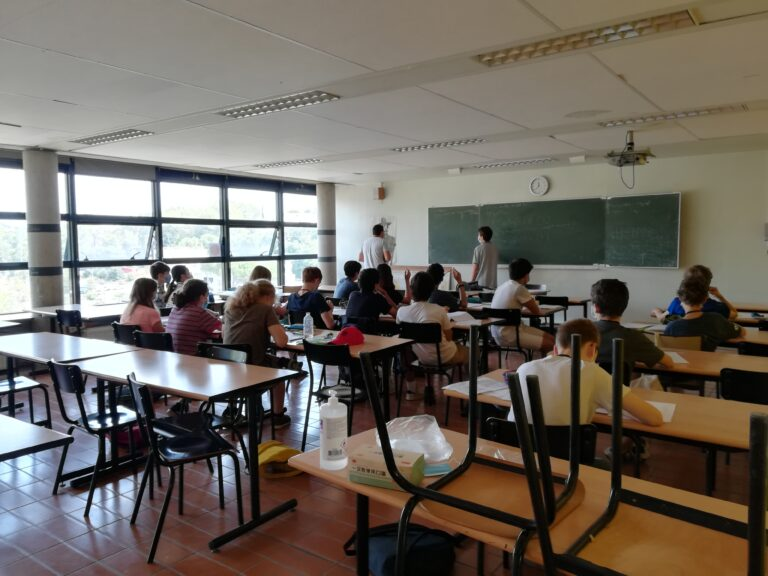
\includegraphics[width=6cm]{CR-23-0.jpg}
\caption{Réussirez-vous à trouver Angela parmi les élèves ?}
\end{figure}

L’après-midi, le groupe A s’entraîne sur le principe de récurrence avec Raphaël, tandis que le groupe B s’amuse à compter le nombre de chemins que peut parcourir une fourmi sur une grille. Équations fonctionnelles et séries génératrices sont au programme pour les groupes C et D (rassurez-vous, les noms font peur, mais en vrai c’est compréhensible !).

\begin{figure}[H]
\centering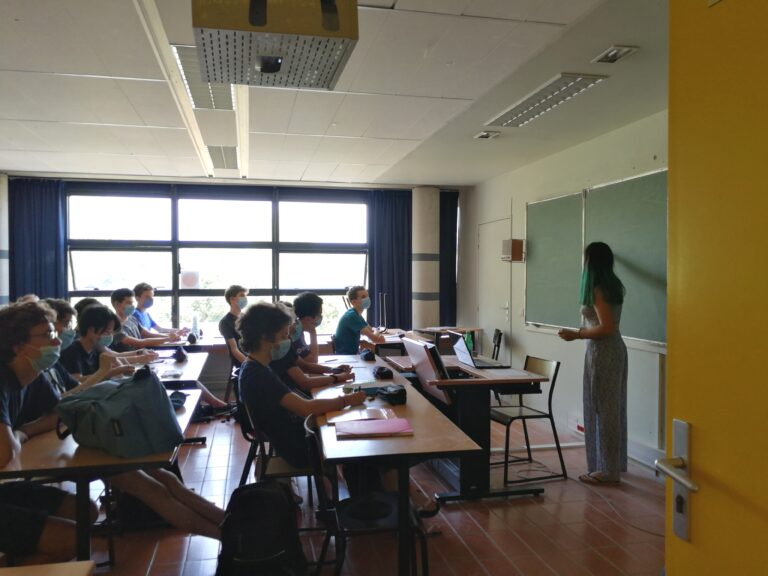
\includegraphics[width=6cm]{CR-23-1.jpg}
\caption{Place au duo Maena et Emile pour le cours de dénombrement au groupe B}
\end{figure}

Mais le plus gros événement de la journée reste le tournage d’un film pour NiceTV sur le site du CIV ! Bien qu’il se déroulait au pied du bâtiment des cours à la plus grande satisfaction des élèves, qui ont pu y assister à la pause, ceci ne les a pas empêché de suivre assidûment les cours.

\begin{figure}[H]
\centering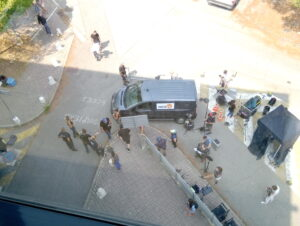
\includegraphics[width=6cm]{CR-23-2.jpg}\hspace{2cm}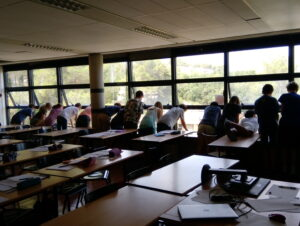
\includegraphics[width=6cm]{CR-23-3.jpg}
\caption{Film d’action, policier, d’auteur… ? Les élèves assistent au tournage.}
\end{figure}

La journée s’est terminée encore une fois par des séances de volley et de foot, mais aujourd’hui la piscine était ouverte donc de nombreux intéressés se sont vite jetés à l’eau. Après manger, soirée calme pour les élèves en prévision de l’entraînement de demain.

\begin{figure}[H]
\centering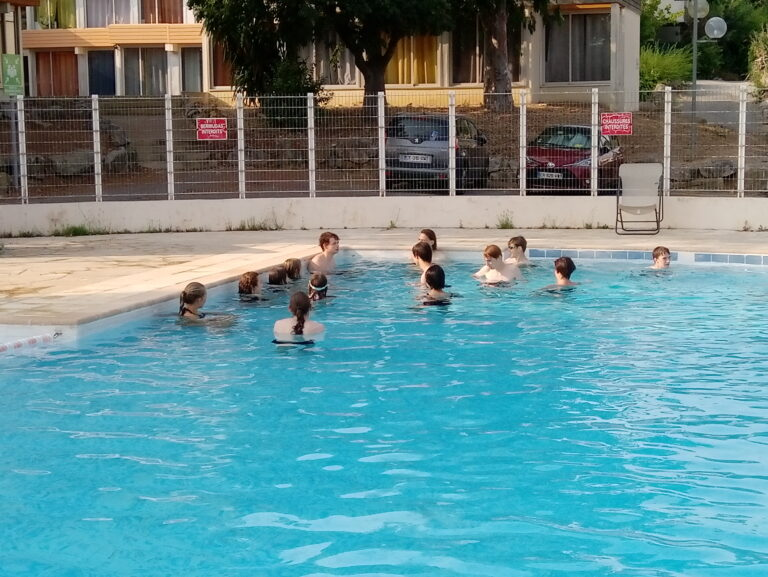
\includegraphics[width=6cm]{CR-23-4.jpg}
\caption{Rien de mieux qu’une bonne baignade pour supporter la chaleur du sud}
\end{figure}